\section{Experimento}

\begin{frame}
  \frametitle{Amostragem}
  \begin{itemize}
	  \item Residencial (\ang{+5;35;2.00} e \ang{-0;11.;58}):
	  Avenida com pouco tráfego de veículos e não pavimentada
  \item Tráfego (\ang{+5;34;54} e \ang{-0;11;56.30}):
	  Avenida pavimentada com tráfego intenso de veículos (com exceção do período noturno).
  \end{itemize}
\end{frame}

\begin{frame}
  \frametitle{Pontos de amostragem em Nima}
  \begin{figure}[H]
    \centering
    \caption{Amostragem Nima}
    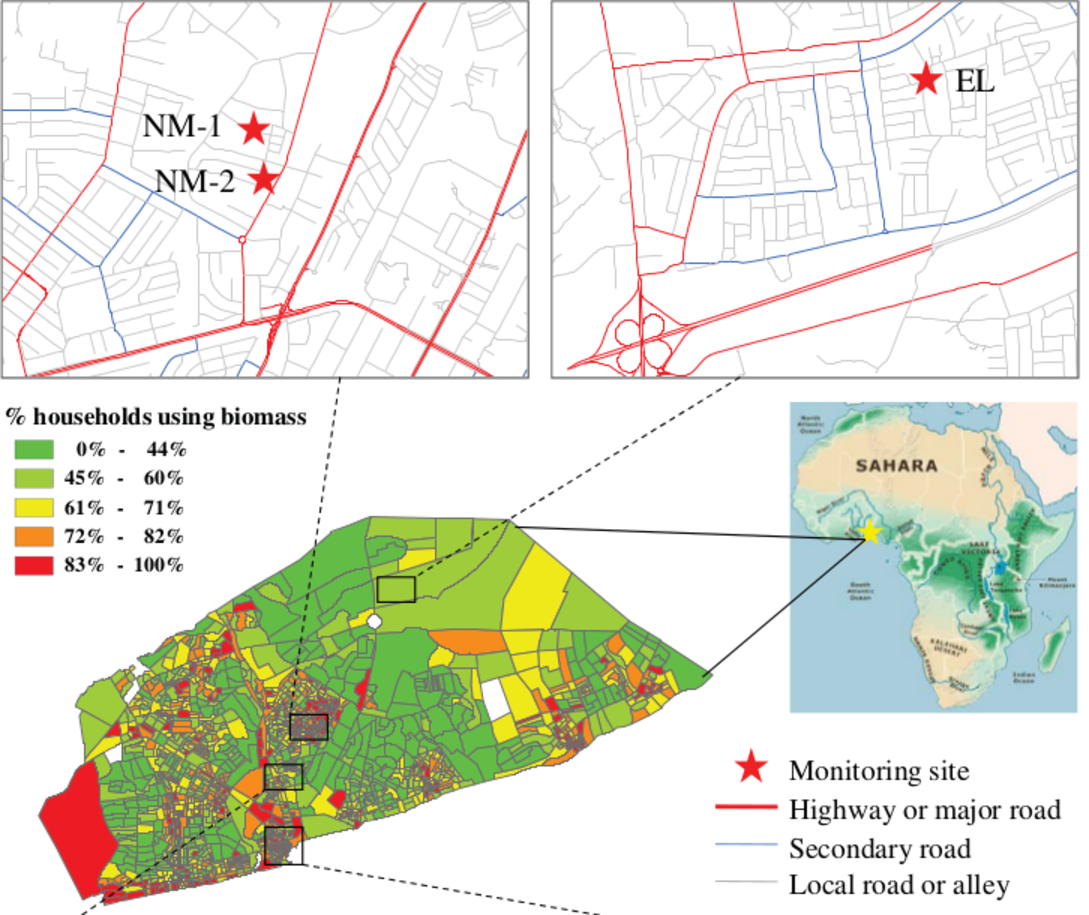
\includegraphics[scale=0.35]{../../../inputs/zheng_images/nima_mapa.pdf}
  \end{figure}
\end{frame}

\begin{frame}
  \frametitle{Etapas}
  \begin{itemize}
    \item Adaptações no sistema de Fluorescência de Raios-X (EDX) disponível no Lapat, 
          para ajustá-lo à irradiação de filtros de Teflon
    \item Análise das 2897 amostras de Gana
    \item Integração dos espectros
    \item Aperfeiçoamento do software de cálculo das concentrações (em linguagem C)  
    \item 4 Calibrações do EDX (250 amostras)
    \item Refletância para Black Carbon
    \item Organização dos dados finais para análise estatística: Positive Matrix Factorization (PMF)
	  e análise multivariada.
 \end{itemize}
\end{frame}

\begin{frame}
  \frametitle{Calibração linha K}
  \begin{figure}[H]
    \centering
    \caption{Calibração}
    \includegraphics[scale=0.35]{../../../outputs/limitDetectionK.pdf}
  \end{figure}
\end{frame}

